\documentclass[11pt]{article}

\usepackage{graphicx}

% Enable references to labels in the notes
\usepackage{xr-hyper} \externaldocument{p328_notes}
\usepackage{hyperref}

% Sans fonts
\usepackage{sfmath} \renewcommand{\familydefault}{\sfdefault}

\newcommand{\COURSE}{PHYS328W} \newcommand{\LABNUM}{1}
\newcommand{\TITLE}{Voltage Dividers} \markright{\COURSE~Lab
  \LABNUM\ : \TITLE}

\setlength{\textwidth} {6.5 true in} \setlength{\textheight}{9 true
  in} \setlength{\hoffset} {-0.75 true in} \setlength{\voffset} {-0.75
  true in} \setlength{\parindent} {12 pt} \pagestyle{myheadings}

\begin{document}

\thispagestyle{empty}

\section*{\COURSE\ Lab \LABNUM\ : \TITLE}

This assignment relies on Sections~\ref{sec:ohm} and \ref{sec:serpar}
of the notes.

\subsection*{Experiments}

\begin{figure}[h]
\centering 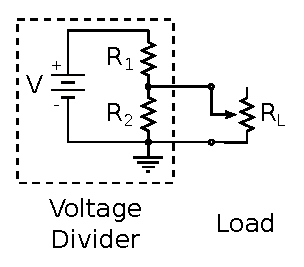
\includegraphics{vdivider.eps}
\caption{A voltage divider driving a variable load resistor $R_L$.}
\label{fig:vdivider}
\end{figure}

\begin{enumerate}
\item Find two unequal resistors in the 100~$\Omega$ - 1~k$\Omega$
  range and 10~k$\Omega$ potentiometer (pot).

\item Use a Digital Multimeter (DMM) to measure the resistances of the
  resistors.

  \emph{A guide to using a DMM to make measurements is in
    Appendix~\ref{sec:dmm} of the notes.}

\item Construct the voltage divider circuit shown in
  Figure~\ref{fig:vdivider} using the 5~V source on your prototyping
  board. The three pins of the pot are spaced so that you can plug
  them into three adjacent (numbered) rows on the breadboard, enabling
  you to use several (lettered) sockets to connect resistors and
  wires to them. You will only using the middle pin and one of the
  outer pins of the pot. The middle pin is represented by
  the arrow in the schematic symbol.

  \emph{The layout of the connections between sockets on a
  breadboard is shown in Figure~\ref{fig:breadboard} in
  Appendix~\ref{sec:breadboard} of the notes.}

\item The voltage $V_{out}$ across the load resistor $R_L$ is the
  output voltage of the divider. Measure $V_{out}$ for 10 values of
  $R_L$ covering the range of the pot. Each time you change $R_L$, you
  will need to disconnect one of the leads to the potentiometer and
  measure its resistance with the DMM.

  \emph{Your 10 values of the load resistance need not be evenly
    spaced. You should find that there is a range of $R_L$ values
    over which $V_{out}$ changes very little. Choose your $R_L$ values
    strategically to cover the range where $V_{out}$ is changing
    significantly.}

\item Also record the open-circuit value of $V_{out}$. This is the
  value of $V_{out}$ with no load (infinite load resistance). To
  measure this, disconnect either pin of the pot (or both) from the
  circuit.

\item Record all of your measurements in your log book.
\end{enumerate}

\subsection*{Calculations}

In your log book ...

\begin{enumerate}
\item Choose two of the values of $R_L$ that you measured --- the
  largest and the one closest to $R_2$, and use the equivalent
  resistance and current division equations
  (Equations~\ref{eq:Rseries}, \ref{eq:Rparallel}, and \ref{eq:Idiv}
  of the notes) along with your measured resistances to calculate the
  current flowing through the load. From that, find $V_{out}$.

\item Use a voltage division equation (Equation~\ref{eq:Vdiv} of the
  notes) to predict the open-circuit value of $V_{out}$.
\end{enumerate}

\subsection*{Products}

Upload to Canvas the PDF of a brief \LaTeX\ report in which you
discuss the degree of agreement between your measurements and
theoretical predictions of the behavior of the voltage
divider. Include as a figure a graph of measured and theoretical
output voltage vs. load resistance. Comment on any lesson(s) you draw
from your results with respect to designing voltage dividers.

\end{document}
